% Draft for internal discussion (advisor meeting). Compile on Overleaf with pdfLaTeX + BibTeX.
% Figures are generated by paper/make_figures.py; references by paper/make_bib.py (arXiv API).
\documentclass[11pt]{article}

\usepackage[margin=1in]{geometry}
\usepackage[T1]{fontenc}
\usepackage[utf8]{inputenc}
\usepackage{lmodern}
\usepackage{microtype}
\usepackage{amsmath,amssymb}
\usepackage{booktabs}
\usepackage{multirow}
\usepackage{graphicx}
\usepackage{xcolor}
\usepackage{enumitem}
\usepackage[font=small,labelfont=bf]{caption}
\usepackage[numbers,sort&compress]{natbib}
\usepackage[colorlinks=true,linkcolor=blue!50!black,citecolor=blue!50!black,urlcolor=blue!50!black]{hyperref}

\newcommand{\pending}[1]{\textcolor{red}{[pending: #1]}}
\newcommand{\note}[1]{\textcolor{orange!80!black}{[#1]}}
\newcommand{\chrono}{\textsc{chron}}
\newcommand{\rev}{\textsc{newest}}
\newcommand{\retr}{\textsc{retr}}
\newcommand{\ci}[2]{\,[$#1$,\,$#2$]}
\setlist{nosep,leftmargin=1.4em}

\title{Written Later, Read as Newer:\\Language Models Mistake Presentation Order for Time}
\author{Author Names\\\small Affiliation\\\small\texttt{email@example.org}}
\date{Draft, October 2026 --- for internal discussion}

\begin{document}
\maketitle

\begin{abstract}
When a context states several values of the same quantity---a variable rewritten in a chain of thought, a user's city across chat sessions, a setting across commits---a language model must decide which value is current.
We show that open models largely decide by position: the value written last is read as the newest, even when explicit dates, step numbers or ordering statements say otherwise.
In shuffled chains of thought that overwrite a variable eight times, all 14 open models we test (1.7B--14B parameters) answer with the last-presented value in 89.5--99.5\% of items.
On long-term memory benchmarks with dated sessions, showing the sessions newest first costs 18--63 accuracy points; on MemConflict, a third-party conflict benchmark, merely ordering the same sessions by retrieval relevance costs Qwen3-4B 19 points (75.4$\rightarrow$56.2).
The effect is specific: on PersonaMem and on LoCoMo temporal questions, which can be answered without resolving a conflict between an older and a newer state, order has no effect.
We trace two failure points.
In short contexts the model internally represents which value is newer (linear-probe accuracy $\approx$98\%) but does not use it, and misleading order is copied into the model's own reasoning and then read by position.
In long sessions, dates written in session headers are not bound to the facts they govern.
Accordingly, two training fixes that never see the test formats address the two points: training on records whose presentation order is decoupled from time repairs \emph{selection} (newest-first logs 70$\rightarrow$100; step-numbered chain of thought 6$\rightarrow$75), and training to bind facts to distant dates repairs \emph{binding} (held-out ConvoMem-long 77$\rightarrow$96), even when the binding data are always chronological.
Prompting, explicit ordering statements and thinking mode do not help.
\end{abstract}

% =====================================================================
\section{Introduction}

Much of what language models read is a record of change.
A chain of thought (CoT) assigns a value and later revises it; a chat assistant's memory holds the user's address before and after a move; a log lists the successive values of a configuration key.
To answer ``what is the value now?'', a reader must order these statements in time.
In most training text this is trivial, because text is written in the order events happen: the statement written last is also the most recent.
\emph{Later in the text} is therefore an excellent proxy for \emph{later in time}.

Many contexts that models read at deployment break this proxy.
E-mail clients, \texttt{git log}, changelogs and feeds list the newest entry first.
Retrieval-augmented memories return passages by relevance, not by date.
Agents append retrieved memories after their own trajectory; monitors read other models' reasoning out of order; tools concatenate outputs from many sources.
In all of these, time is usually still \emph{written down}---as a date, a timestamp or a step number---but it disagrees with the order of presentation (Figure~\ref{fig:concept}).

This paper asks a simple question: \textbf{when presentation order and explicit time disagree, which one does a language model follow?}
Standard benchmarks cannot answer it, because they present updates chronologically, so that a reader who uses dates and a reader who uses position give the same answer (\S\ref{sec:setup}).
We therefore hold the content fixed and vary only the order, across controlled chains of thought, deployed formats, and third-party long-term memory benchmarks.

\begin{figure}[t]
  \centering
  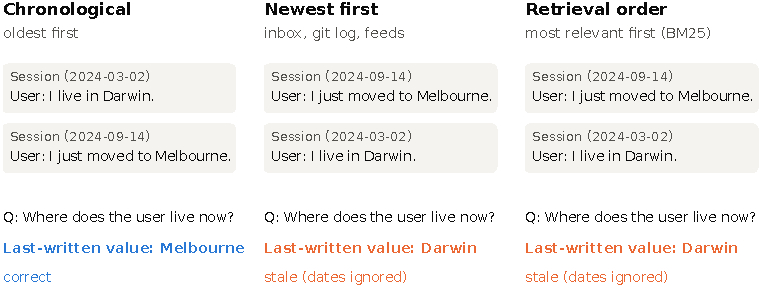
\includegraphics[width=\linewidth]{figures/fig1_concept.pdf}
  \caption{\textbf{Order versus time.} The same two dated sessions shown in three orders (schematic example). A reader that takes the last-written value as current answers correctly only under chronological presentation. Newest-first lists and retrieval-ranked memories are common at deployment; the dates are present in all three cases.}
  \label{fig:concept}
\end{figure}

Our findings are:
\begin{enumerate}
  \item \textbf{Position wins over explicit time.} In shuffled chains of thought, readers answer with the last-presented value in 89.5--99.5\% of items once a variable is overwritten eight times; a step number on every line or a ``listed from most recent'' header rarely overrides this (except for Qwen3-14B on short, well-structured lists), and an explicit retraction (``Wait, that's wrong.'') only partly offsets it (\S\ref{sec:cot}).
  The same default appears in deployed formats: showing dated LongMemEval sessions newest first costs 24--53 points, and stating that the sessions are ordered newest first recovers at most 2.6 (\S\ref{sec:apps}).
  \item \textbf{It reproduces on third-party benchmarks, and natural retrieval order triggers it.} On MemConflict \citep{tao2026memconflict}, Qwen3-4B drops from 75.4\% to 36.2\% when sessions are shown newest first, and to 56.2\% when they are shown in BM25 relevance order---an order that a standard retrieval memory produces without any adversarial intervention (\S\ref{sec:external}).
  \item \textbf{It is specific to conflicting states.} On PersonaMem \citep{jiang2025personamem} and LoCoMo \citep{maharana2024locomo} temporal questions, order has no effect. Diagnostics show that these questions do not require choosing between an older and a newer state (PersonaMem's update questions can even be answered without the history), consistent with our CoT finding that order matters only when a state is overwritten (\S\ref{sec:boundary}).
  \item \textbf{Two failure points.} In short contexts the failure is one of \emph{selection}: the newer value is linearly decodable at the answer position in $\approx$98\% of items, including those the model answers with the stale value, and the misleading order is copied into the model's own timeline or thinking, which it then reads by position. In long sessions the failure is one of \emph{binding}: dates in session headers are not attached to facts that appear thousands of tokens later (\S\ref{sec:mechanism}).
  \item \textbf{Two fixes, validated on unseen formats.} Training on synthetic records whose presentation order is decoupled from time (no chat, log, or CoT formats) repairs selection and transfers to newest-first logs, to step-numbered CoT and to the model's own lists, whereas an identical chronological-only control does not. Training on long block-dated documents to bind facts to distant dates repairs reading of held-out conversations; here the chronological-only control works as well, so the active ingredient is binding rather than decoupling (\S\ref{sec:fix}).
\end{enumerate}

For the training study and for every experiment after the initial chain-of-thought study, we wrote a numerical threshold before running it; we report all outcomes, including the many that did not meet their thresholds (Appendix~\ref{app:scorecard}).

% =====================================================================
\section{Related work}
\label{sec:related}

\paragraph{Order and position in context.}
Models use information at the beginning and end of long contexts better than in the middle \citep{liu2024lost}, and permuting premises hurts reasoning \citep{chen2024premise}.
Studies of shuffled chains of thought report that answers often survive shuffling \citep{lca2026,cotorder2026a} while small models read arithmetic CoT by copying numbers by position \citep{cotorder2026b}; our CoT experiments reconcile these results: order matters exactly when a state is overwritten.
For many in-context updates of a key--value list, retrieval of the latest value degrades and early values intrude \citep{qiao2026retrieval,chattaraj2026first}; with up to 64 overwrites inside a chain of thought we instead observe a stable recency default.
\citet{fitch2026gemma} find that source framing outweighs position for two short conflicting documents, with a primacy rather than a recency bias for Gemma; \citet{fatemi2024tot} show that fact order affects temporal reasoning; and in-context retrieval shows recency and contiguity biases reminiscent of human episodic memory \citep{temporalbias2025}.
When recency and another cue are perfectly correlated in training, which rule a model adopts is not determined by the data \citep{liao2026shortcut}; this is why we make the cues conflict.
None of these studies pits presentation order against explicit time.

\paragraph{Knowledge updates and stale state.}
Entity tracking has been studied with box-moving tasks \citep{kim2023entity}; \citet{tang2026entities} find that models do not update world states step by step but aggregate the relevant statements at query time, and fail when the order of operations matters.
Concurrently, \citet{guo2026context} characterize ``stale binding'' when a variable is updated in context: the current value remains decodable, attention drifts to older values, and an attention bias at known positions repairs the answer. Their updates are always presented chronologically and the fix requires knowing where the current value is; we study the conflict between order and explicit time, show the failure is copied into the model's own reasoning, separate selection from binding in long sessions, and fix both without position information.
Outdated retrieved documents can override correct parametric answers, and dates alone barely help \citep{ahmed2026stale}; temporal conflicts across document versions mislead models \citep{ozer2025temporal}; and masking superseded records in the KV cache shifts preference toward new values at a cost in detail \citep{zhou2026positions}.
On the generation side, reflection markers such as ``wait'' behave as surface cues \citep{yu2026markers}; we find a similar weakness of retraction markers on the reading side.

\paragraph{Long-term memory.}
LongMemEval \citep{wu2025longmemeval} includes knowledge-update questions and sorts retrieved sessions by timestamp by default; we quantify the cost of not doing so.
MemConflict \citep{tao2026memconflict} evaluates memory systems under dynamic, static and conditional conflicts but does not vary presentation order.
RoutePrism \citep{xu2026routeprism} varies the order in which records are \emph{ingested} into a memory and shows that retention policies then keep different evidence; our effect arises with all evidence present.
\citet{jiang2026render} show that much of the gain of structured memories comes from a readable, time-ordered rendering, in line with our results.
Memory systems add explicit state labels \citep{shi2026atma} or temporal indexes \citep{liu2026segtree}, and Supersede \citep{patel2026supersede} trains a bounded-memory agent to keep current values, noting that frontier models resolve explicit updates by a last-mention scan---the heuristic we show fails out of chronological order.

% =====================================================================
\section{Setup}
\label{sec:setup}

\paragraph{Formalization.}
A context contains records $r_1,\dots,r_n$ about one queried quantity. Record $r_i$ carries a value $v_i$ and a time $\tau_i$ that is \emph{written in the text} (a date, a timestamp, or a step number), and the records are presented in an order given by a permutation $\pi$, where $\pi(i)$ is the position of $r_i$. The current value is
\begin{equation}
  v^\star = v_{i^\star}, \qquad i^\star = \arg\max_i \tau_i .
\end{equation}
Two idealized readers answer differently:
\begin{equation}
  f_{\text{time}}(r,\pi) = v_{\arg\max_i \tau_i}, \qquad
  f_{\text{pos}}(r,\pi) = v_{\arg\max_i \pi(i)} .
\end{equation}
They agree whenever $\pi$ is increasing in $\tau$, which is the case in almost all naturally written text and in standard benchmarks. We therefore compare the same records under several orders:
\chrono{} (oldest first, $\pi$ increasing in $\tau$), \rev{} (newest first, $\pi$ decreasing in $\tau$), shuffled, and \retr{}, in which records are sorted by a BM25 relevance score $s(q, r_i)$ to the question $q$, most relevant first:
\begin{equation}
  \pi_{\text{retr}}(i) < \pi_{\text{retr}}(j) \iff s(q,r_i) > s(q,r_j).
\end{equation}
\retr{} is not chosen by us: it is the order a standard retrieval memory hands to the reader.

\paragraph{Measures.}
We report accuracy and the \emph{stale rate} (the answer is a superseded value).
The \emph{order effect} is the paired difference $\Delta = \mathrm{Acc}(\textsc{order}) - \mathrm{Acc}(\chrono)$ over the same items, with a 95\% paired bootstrap interval (10{,}000 resamples of items).
Free-text answers are graded by Qwen3-14B (4-bit) given the question, the reference answer and, where available, the older and newer evidence, choosing among \emph{up to date}, \emph{stale}, and \emph{other}; agreement with string matching on the items where it applies is 91.4\% on LongMemEval and 90.8\% on MemConflict.

\paragraph{Models.}
Chain-of-thought experiments use 14 open models: Qwen3-1.7B/4B/4B-Base/8B/14B \citep{qwen3}, OLMo-2-7B (Base, SFT, DPO, Instruct) and OLMo-2-13B (Base, Instruct) \citep{olmo2}, Qwen2.5-Math-7B, DeepSeek-R1-Distill-Qwen-7B \citep{deepseekr1}, and Phi-4-mini-instruct \citep{phi4mini}. Models of 7B parameters and above run in 4-bit. Application experiments focus on Qwen3-4B, Qwen3-14B and Phi-4-mini, in non-thinking mode with greedy decoding unless stated.

\paragraph{Protocol.}
For the training study (pre-registered) and for all experiments after the initial chain-of-thought study, we wrote the hypothesis and a numerical threshold before running; in the chain-of-thought study, task categories and conditions were fixed in code before running. Controls differ from treatments in exactly one variable.
Test sets used to design a fix are never used to evaluate it.
LongMemEval was used to discover the phenomenon and is reported as \emph{seen}; ConvoMem personas 50--99, ConvoMem-long, PersonaMem, MemConflict and LoCoMo are held out.
Table~\ref{tab:sets} lists the test sets.

\begin{table}[t]
\centering\small
\caption{\textbf{Test sets.} ``Conflict'': the question requires choosing between an older and a newer state of the same quantity. Orders: C = chronological, N = newest first, S = shuffled, R = BM25 retrieval order.}
\label{tab:sets}
\begin{tabular}{@{}lllccl@{}}
\toprule
Set & Source & Length (tokens) & Conflict & Orders & Status \\
\midrule
Variable tracking in CoT & ours (synthetic) & 16--72 lines & yes & C, S, N & -- \\
BBH, model's own CoT (26 tasks) & \citet{suzgun2023bbh} & short & varies & C, S & -- \\
LongMemEval knowledge update (78) & \citet{wu2025longmemeval} & 4.1k--9.3k & yes & C, N & seen \\
E-mail threads, git log, CHANGELOG & ours (synthetic) & 0.5k--8.4k & yes & C, N & -- \\
Agent trajectories + memory & ours (synthetic) & short & yes & placement & -- \\
ConvoMem-long (124) & \citet{convomem2025} & 2.4k (median) & yes & C, N & held out \\
MemConflict, dynamic (240) & \citet{tao2026memconflict} & 6.7k--21.7k & yes & C, N, R & held out \\
PersonaMem 32k (589) & \citet{jiang2025personamem} & 16k--30k & no & C, N & held out \\
LoCoMo temporal (321) & \citet{maharana2024locomo} & 13k--25k & no & C, N, R & held out \\
MemoryAgentBench CR (76) & \citet{hu2025memoryagentbench} & 6.9k & counterfactual & C, N, R & seen \\
\bottomrule
\end{tabular}
\end{table}

% =====================================================================
\section{Position is read as time}
\label{sec:phenomenon}

\subsection{Chains of thought}
\label{sec:cot}

\paragraph{Shuffling hurts only overwritten state.}
We generate 16-line programs whose CoT assigns the queried variable $k$ times, and ask the reader for its final value after the CoT lines are shuffled (Figure~\ref{fig:cot}a; Qwen3-4B, $n=200$ per cell).
Variables assigned once are read correctly after shuffling ($\geq$99.5\%), but accuracy on overwritten variables falls to 79.5/39.5/19.0/14.0\% at $k=1/2/4/8$, close to chance among the $k{+}1$ candidates.
The reader is not guessing: it picks the value presented last in 93.5--98.5\% of items for $k \geq 2$, and in 93--99\% of items in a longer variant with up to $k=64$ overwrites, where the first-presented value is never chosen for $k \geq 2$.
At $k=8$, all 14 models pick the last-presented value in 89.5--99.5\% of shuffled items, while variables assigned once stay above 96.8\%. Larger models resist at small $k$ (at $k=2$: Qwen3-14B 73.5\%, OLMo-2-13B-Instruct 87.0\%) but not at $k=8$ (97.0\% and 95.0\%). Base, SFT, DPO and RL-tuned OLMo-2-7B checkpoints behave alike (93.5--99.0\% at $k=8$), and a natural-language version (``Box E has 41 marbles'') behaves identically.
On the model's own reasoning for all usable BBH tasks, shuffling breaks 39\% of answers on tasks that we labeled in advance as tracking updated state, and 4\% on the others.
This reconciles reports that shuffled CoT preserves answers \citep{lca2026,cotorder2026a} with reports that it does not \citep{cotorder2026b}: order matters exactly when a state is overwritten.

\begin{figure}[t]
  \centering
  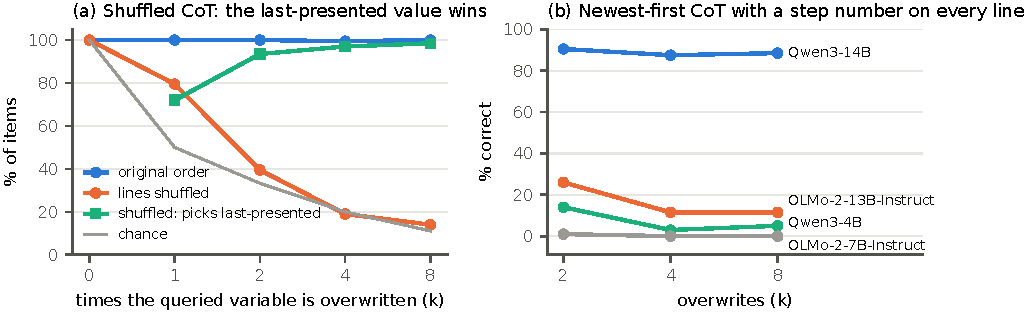
\includegraphics[width=\linewidth]{figures/fig2_cot.pdf}
  \caption{\textbf{Chain-of-thought readers take the last-presented value.} (a) Qwen3-4B on a synthetic 16-line program whose CoT overwrites the queried variable $k$ times ($n=200$ per point). After shuffling, accuracy falls to chance because the reader picks whichever value is presented last. (b) Newest-first CoT with an explicit step number on every line; accuracy in the conflict case, where position points to a stale value. Only Qwen3-14B uses the step numbers.}
  \label{fig:cot}
\end{figure}

\paragraph{Explicit order cues lose to position.}
When the CoT lines are listed newest first with a step number on every line (Figure~\ref{fig:cot}b), Qwen3-4B answers correctly in 3--14\% of conflict cases, OLMo-2-13B-Instruct in 11.5--26\% and OLMo-2-7B-Instruct in 0--1\%; only Qwen3-14B uses the numbers (87.5--90.5\%).
A header stating that the list is ``most recent first'' is worse still (Qwen3-4B: 0--1\%).
A retraction marker attached to the wrong value (``$t = 51$. Hmm, that's wrong.'') helps but does not override position: when the retracted value comes last, Qwen3-4B still picks it in 60--80\% of items, and the best model (Qwen3-14B) reaches 47.5\% accuracy.
In real reasoning traces (OpenR1-Math) with two counterfeit conclusions, the earlier one A and a later one B followed by ``Wait, that's wrong.'', a rational reader should choose A; with 10\% of the derivation kept, readers still choose the retracted B at least as often (Qwen3-4B 56.5\% vs.\ 19.4\%, Qwen3-14B 45.5\% vs.\ 27.5\%, OLMo-2-13B-Instruct 41.5\% vs.\ 40.0\%).
Reading its own unedited reasoning, by contrast, Qwen3-4B is accurate (93--100\% on most BBH tasks): the positional default is usually right for text written in chronological order.

\subsection{Deployed formats}
\label{sec:apps}

\paragraph{Chat memory.}
We take the 78 knowledge-update questions of LongMemEval, each with two dated sessions (4.1k--9.3k tokens) in which the later session updates a fact from the earlier one, and present the sessions oldest or newest first (Figure~\ref{fig:apps}a).
Newest first costs Qwen3-4B 25.6 points (76.9$\rightarrow$51.3), Qwen3-14B 24.4 and Phi-4-mini 52.6; stale answers rise to 41, 36 and 59\%. All intervals exclude zero.
Adding ``the sessions are listed from the most recent to the oldest'' recovers 0--2.6 points; removing the dates makes things worse, so the dates are used, but weakly.

\paragraph{Logs and agent memory.}
In synthetic e-mail threads, git logs and changelogs in which every entry is dated, newest-first presentation costs 12.1\ci{8.6}{15.6} points for Qwen3-4B, 27.4 for OLMo-2-13B-Instruct and 31.4 for Phi-4-mini, and only 3.9 for Qwen3-14B in these short (0.8k-token) contexts. E-mail threads are hardest: Qwen3-4B drops from 88.3\% to 58.0\%, Phi-4-mini from 86.3\% to 15.0\%.
In agent trajectories, inserting a retrieved, explicitly time-stamped stale memory right before the question lowers Qwen3-4B accuracy by 9.7 points (k = 3 updates: 88.7$\rightarrow$69.3), while the same memory at the beginning of the context is harmless ($-$0.7): what matters is where the stale value sits.

\begin{figure}[t]
  \centering
  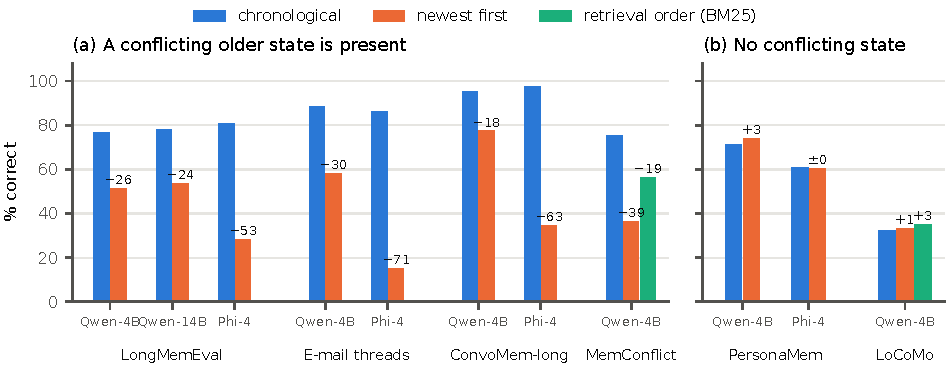
\includegraphics[width=\linewidth]{figures/fig3_apps.pdf}
  \caption{\textbf{Order effects in deployed formats and third-party benchmarks.} Numbers above bars are differences from the chronological bar. (a) When an older, conflicting state is present, newest-first presentation costs 18--71 points, and BM25 retrieval order costs 19 points on MemConflict. LongMemEval and e-mail numbers from \S\ref{sec:apps}; ConvoMem-long, MemConflict from \S\ref{sec:external}. (b) PersonaMem and LoCoMo temporal questions, which do not require resolving such a conflict, show no order effect (\S\ref{sec:boundary}).}
  \label{fig:apps}
\end{figure}

\subsection{Held-out benchmarks and retrieval order}
\label{sec:external}

\paragraph{ConvoMem-long.}
From ConvoMem's changing-evidence questions \citep{convomem2025} we take personas 50--99 (never used in any design decision) and the full 40-message conversations (median 2.4k tokens), date the two conversations in their source order, and present them oldest or newest first. Newest first changes Qwen3-4B's accuracy by $\Delta = -17.7$\ci{-25.0}{-10.5} points (95.2$\rightarrow$77.4) and Phi-4-mini's by $-62.9$\ci{-71.8}{-54.8} (97.6$\rightarrow$34.7).

\paragraph{MemConflict.}
MemConflict simulates users whose state changes over four years of monthly sessions and asks, after each update, how an attribute changed.
We use the 240 dynamic-conflict questions (at most 8 per simulated user) in which the old value is \emph{not} restated in the update session but appears in an earlier one, so that the answer requires relating two sessions by their dates.
Each context contains the earlier session, the update session, and the sessions just before the update (2--6 sessions; median 18.5k tokens), each headed by its date.
Qwen3-4B answers 75.4\% correctly in chronological order, 36.2\% newest first ($\Delta = -39.2$\ci{-46.2}{-31.7}) and 56.2\% in BM25 retrieval order ($\Delta = -19.2$\ci{-25.4}{-13.3}); the share of answers that state the change in the wrong direction rises from 5.0\% to 37.9\% and 18.3\%.
Retrieval order places the update session first in 86 of 240 items; accuracy is 48.8\% on these and 60.4\% on the rest.
Since the retrieved sessions are the same in both conditions, re-sorting retrieved memories by their timestamps before reading recovers the full 19 points at no cost.

\subsection{Where order does not matter}
\label{sec:boundary}

\paragraph{PersonaMem and LoCoMo.}
On the 238 PersonaMem questions about how a preference evolved and why it changed (16k--30k tokens), presenting sessions newest first has no effect (Qwen3-4B $+2.5$\ci{-0.8}{5.9}; Phi-4-mini $-0.4$\ci{-3.8}{2.9}); the same holds for the five other question types (largest drop $-5.9$, $n=17$), and for the 321 LoCoMo temporal questions ($+1.2$\ci{-3.7}{5.9} newest first, $+3.1$\ci{-1.6}{7.8} in retrieval order).
Diagnostics explain why (Appendix~\ref{app:pmdiag}).
PersonaMem's update questions can be answered without the history: matching words between the user's final message and the options alone selects the correct option for 80.8\% of the ``why did the preference change'' questions (Qwen3-4B with the full history: 83.8\%), and Phi-4-mini answers ``how did the preference evolve'' questions equally well with and without the history (51.8\% both).
The remaining question types do depend on the history, but none requires choosing between an older and a newer state; neither do LoCoMo's temporal questions, which ask when an event happened.
These null results delimit the phenomenon rather than contradict it: order matters when a conflicting older state is present and time is expressed only by position or by dates far from the facts.

\paragraph{A confound.}
On MemoryAgentBench's conflict-resolution facts \citep{hu2025memoryagentbench}, where the newer fact is counterfactual and the older one is world knowledge, Qwen3-4B picks the older fact in 83\% of chronological items: parametric knowledge dominates and the set cannot test order (it was also used in our pre-registered training evaluation, so we treat it as seen).

% =====================================================================
\section{Why: two failure points}
\label{sec:mechanism}

\subsection{Misleading order is copied into the model's own reasoning}
A natural defense is to let the model reason first. It does not help, because the reasoning inherits the presentation order.

\paragraph{Prefilled timelines.}
We write a correct, dated timeline of the two pieces of evidence into the model's response and let it only produce the final answer (Qwen3-4B, Qwen3-14B, $n=70$).
When the timeline lists the evidence newest to oldest and the input is newest first, both models still answer the stale value in about 40\% of items (40.0\% and 38.6\%; Phi-4-mini: 57.1\%), although every date in the list is correct; with an oldest-to-newest list the rate falls to 27.1\% and 10.0\%. Left to their own devices, models mostly list evidence in presentation order.

\paragraph{Swapping thoughts.}
In thinking mode on LongMemEval, Qwen3-4B answers 80.8\% correctly from chronological input and 55.1\% from newest-first input (Figure~\ref{fig:mech}a).
Its thinking restates the evidence in presentation order: among traces that mention both session dates, the newer date comes first in 82.1\% of newest-first runs and 3.6\% of chronological runs.
Swapping the thinking between runs swaps the accuracy: newest-first input with the thinking from the chronological run gives 80.8\%; chronological input with the thinking from the newest-first run gives 57.7\%; removing the input entirely changes little (75.6\% and 52.6\%).
The answer follows the thinking, and the thinking has absorbed the misleading order.
In e-mail threads, thinking fixes the order in short contexts (10 messages: 93.3\% correct newest first) but not in longer ones (200 messages: 53.3\%), where the last value mentioned in the thinking is the newest one in only 51.7\% of items.

\begin{figure}[t]
  \centering
  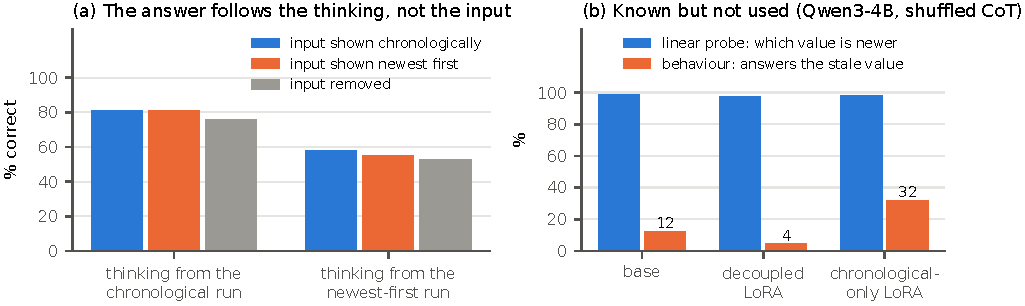
\includegraphics[width=\linewidth]{figures/fig4_mech.pdf}
  \caption{\textbf{Mechanism.} (a) Qwen3-4B in thinking mode on LongMemEval ($n=78$): accuracy depends on which run the thinking comes from, not on the order of the input it is paired with, or on whether the input is shown at all. (b) On shuffled, step-numbered CoT, a linear probe at the answer position decodes which value is newer in $\approx$98\% of items for the base model and both LoRA variants; behavior differs widely. Training changes use, not knowledge.}
  \label{fig:mech}
\end{figure}

\subsection{Short contexts: known but not used}
We train linear probes on the residual stream at the last token before the answer to predict whether the newer value was presented first (layers selected on training items only; 60/40 split by question).
On shuffled, step-numbered CoT the probe reaches 98.8\% (layer 21), and it decodes the correct order on all 13 items that Qwen3-4B answers with the stale value.
On ConvoMem short dialogues it reaches 97.9\%; Qwen3-14B answers MemoryAgentBench fact pairs stale in 50\% of items while its probe reaches 94\%.
The representation is format-specific: probes transfer across formats at near chance (49--58\%).
In short contexts, the model knows which value is newer and fails to select it.

\subsection{Long sessions: dates are not bound to facts}
In long LongMemEval sessions, the same probe is weak (best layer 68.6\% for Qwen3-4B and 72\% for Qwen3-14B in five-fold cross-validation), suggesting that ``which update is newer'' is not available at the answer position.
Models that we trained to write a dated list before answering (\S\ref{sec:binding}, E12) name both session dates in only 19.2\% of newest-first items; when they do, they answer correctly in 86.7\% of items, otherwise in 46.0\%.
The dates sit in session headers thousands of tokens before the facts they govern, and the model does not attach them.
The information is nevertheless readable: forcing attention onto the newer statement at the answer position, an oracle intervention that requires knowing where the answer is and that we use only as a diagnostic \citep[following][]{guo2026context}, raises newest-first LongMemEval accuracy from 52.9\% to 72.9\% (e-mail threads: 60.7\% $\rightarrow$ 100\%).

% =====================================================================
\section{Fixing selection and binding}
\label{sec:fix}

\subsection{Prompting does not help}
Stating the order (``listed from the most recent to the oldest'') recovers at most 2.6 points on LongMemEval.
Asking the model to first write a timeline sorted by date leaves a 21.8\ci{11.5}{32.1}-point stale-rate gap between newest-first and chronological input.
Thinking mode reaches 52.6\% newest first with a sampled answer (55.1\% with a greedy answer from the same kind of thinking), little better than non-thinking (51.3\%); answering only from the model's own notes gives 52.6\%.
Because the failure lives in the reasoning itself, instructions to reason do not remove it.

\subsection{Selection: decoupled training}
\label{sec:selection}

\paragraph{Data.}
We generate 5{,}000 synthetic training samples (9.4M tokens) in formats that appear in no test: sticky notes, ticket updates, CSV change logs, key--value configuration snapshots, ledgers, sensor reports and meeting minutes.
Each sample updates one attribute $k=1$--$6$ times among distractor records and filler prose (0.3k--9.5k tokens).
Records of the same attribute use templates drawn from one pool, contain no cue words (``now'', ``updated'', ``latest''), and differ only in their dates, written in mixed formats.
Questions ask for the current value (60\%), the earliest value (20\%) or the value as of a date (20\%), so that ``always pick the newest date'' is not a shortcut. In 20\% of samples there are no dates; the answer is then the last record, or the first if the text states that it is ordered newest first.
In the \textbf{decoupled} condition records are presented chronologically, reversed or shuffled (one third each), so position carries no information about time. The \textbf{control} contains the identical samples, always chronological; we verified that the two training sets differ only in record order.

\paragraph{Training and evaluation.}
We fine-tune Qwen3-4B with LoRA \citep{hu2022lora} (rank 16, $\alpha=32$, learning rate $10^{-4}$, one epoch, final checkpoint), computing the loss on answer tokens only.
Hyperparameters were fixed on a development set in two further formats (calendar entries, audit tables) before any test was run; the evaluation scripts were frozen and hashed beforehand.

\paragraph{Results.}
Decoupled training transfers to formats it never saw (Table~\ref{tab:selection}, Figure~\ref{fig:fix}a).
On newest-first logs it reaches 100\% (control 89.3\%, base 70.3\%).
On newest-first chains of thought with step numbers it reaches 74.7\% (control 2.0\%, base 6.0\%), although training contained dates and never step numbers.
It repairs reading of the model's own lists: with a prefilled newest-to-oldest timeline and newest-first input it answers 77.1\% correctly (control 51.4\%; $+25.7$\ci{14.3}{37.1}); when the model writes the timeline itself the gain is $+19.2$\ci{9.0}{29.5}, and Phi-4-mini shows the same pattern ($+27.1$\ci{14.3}{40.0}).
The probe analysis (Figure~\ref{fig:mech}b) shows what changed: all three models represent which value is newer ($\approx$98\%), but the stale rate is 12.2\% for the base model, 4.5\% after decoupled training and 31.8\% after chronological-only training, whose probe still decodes the correct order on 47 of the 48 items it answers stale.
Decoupled training improves the use of a representation the model already has; chronological-only training suppresses it.
Training only on decoupled chains of thought transfers in the other direction, to dated logs ($+28.7$\ci{24.7}{32.9} over its control), suggesting a single skill.
Chronological conditions do not degrade, and GSM8K \citep{cobbe2021gsm8k} accuracy is unchanged (90.4\% base, 92.4\% both LoRAs). On BABILong's two-supporting-facts task (qa2, 2k tokens) \citep{kuratov2024babilong} the chronological-only control loses 21 points (35.3\%$\rightarrow$14.0\%) while the decoupled model does not (40.0\%).

\paragraph{Limits.}
The pre-registered primary endpoint was not met: on newest-first LongMemEval sessions the decoupled model scores 48.7\% (control 44.9\%, base 51.3\%). On TempReason \citep{tan2023tempreason}, which requires matching dates to intervals, decoupled training is 7.0\ci{-11.7}{-2.7} points worse than the control, possibly an over-preference for the latest record. The selection fix works where each record carries its own date; it does not reach long sessions, where the dates are not bound to the facts.

\begin{table}[t]
\centering\small
\caption{\textbf{Selection fix (pre-registered; Qwen3-4B, seed 0).} Accuracy (\%) under non-chronological presentation; $\Delta$ = decoupled $-$ chronological-only control with 95\% paired bootstrap interval. No test format appears in training. MemoryAgentBench and LongMemEval are \emph{seen} (\S\ref{sec:setup}). $^\dagger$Exploratory follow-up (E2), not part of the pre-registered test list.}
\label{tab:selection}
\begin{tabular}{@{}llrrrl@{}}
\toprule
Test & Condition & Base & Control & Decoupled & $\Delta$ \\
\midrule
Logs (git, CHANGELOG, e-mail) & newest first & 70.3 & 89.3 & 100.0 & $+10.7$\ci{8.7}{12.7} \\
CoT, step numbers & newest first & 6.0 & 2.0 & 74.7 & $+72.7$\ci{67.7}{77.7} \\
CoT, step numbers & shuffled & 34.7 & 27.3 & 45.7 & $+18.3$\ci{14.0}{22.7} \\
Prefilled list (new$\rightarrow$old)$^\dagger$ & newest first & 57.1 & 51.4 & 77.1 & $+25.7$\ci{14.3}{37.1} \\
MemoryAgentBench, single hop & shuffled & 42.0 & 57.0 & 70.0 & $+13$\ci{4}{23} \\
MemoryAgentBench, multi hop & newest first & 5.0 & 4.0 & 19.0 & $+15$\ci{8}{23} \\
LongMemEval sessions & newest first & 51.3 & 44.9 & 48.7 & $+3.8$\ci{-3.8}{11.5} \\
Test of Time & shuffled & 28.0 & 29.2 & 32.4 & $+3.1$\ci{-2.9}{9.2} \\
TempReason & newest first & 70.3 & 78.3 & 71.3 & $-7.0$\ci{-11.7}{-2.7} \\
\bottomrule
\end{tabular}
\end{table}

\subsection{Binding: fact--time training}
\label{sec:binding}

\paragraph{Data.}
To teach binding, we generate long documents organized in blocks, each opened by a single date line and followed by 150--1500 tokens of unrelated prose in which the statements are buried at random depths (genres: diary, meeting minutes, lab notebook, status report, field log; no chat, e-mail or log formats).
Questions ask for the value at the end, the first value, the value as of a date, and ``on which date was \emph{attribute} recorded as \emph{value}?'', which trains retrieval from a fact back to its date.
The target is a dated list of the relevant records, oldest to newest, followed by the answer.
We again train a decoupled version (blocks in chronological, reversed or shuffled order) and a control whose blocks are always chronological, with identical samples (2{,}500 each, median 2.8k tokens, plus 1{,}000 samples with local dates from an earlier run).

\paragraph{Results.}
On held-out ConvoMem-long conversations, newest-first accuracy rises from 77.4\% to 95.2\% with decoupled binding training and to 96.0\% with the chronological-only control (Table~\ref{tab:binding}); chronological accuracy rises as well.
Both models write the two conversation dates in most answers (97.6\% and 88.7\%) and, when they do, list them oldest first (100\% and 97.3\%).
The difference between the two arms is $-0.8$\ci{-5.6}{4.0}: the gain comes from binding, not from decoupling.
This contrasts with an earlier version of the same idea (E12) whose training data placed dates next to each record: there, the chronological-only control learned to restate evidence in presentation order (only 17\% of its lists were sorted) and fell to 25.6\% on newest-first LongMemEval.
Once each fact is written down with its own date, the reader orders facts by date rather than by position.
On LongMemEval (seen) binding training raises the share of answers that name both session dates from 19.2\% to 82.1\% and accuracy from 51.3\% to 62.8\%, still 18 points below chronological presentation.
On MemConflict, the held-out test of this hypothesis, results are \pending{E13 decoupled and control on MemConflict, queued for 10-05 02:00}.

\paragraph{Cost.}
Writing the list first hurts in very long contexts: on PersonaMem (25k tokens), where order does not matter, decoupled binding training lowers accuracy by 11--18 points, 14\% of answers being truncated at the 320-token budget. On long e-mail threads it is slightly worse than the selection fix (200 messages newest first: 73.3\% versus 88.3\% for E12 and 100\% for the answer-only LoRA). An answer-only variant of binding training is in progress \pending{E13b}.

\begin{table}[t]
\centering\small
\caption{\textbf{Binding fix (Qwen3-4B, seed 0).} Accuracy (\%). Binding data contain no chat formats. $\Delta$ vs.\ base with 95\% paired bootstrap interval.}
\label{tab:binding}
\begin{tabular}{@{}llrrrl@{}}
\toprule
Test & Order & Base & Binding, chron.\ only & Binding, decoupled & $\Delta$ (decoupled) \\
\midrule
ConvoMem-long (held out) & chronological & 95.2 & 99.2 & 100.0 & $+4.8$\ci{1.6}{8.9} \\
ConvoMem-long (held out) & newest first & 77.4 & 96.0 & 95.2 & $+17.7$\ci{10.5}{25.0} \\
MemConflict (held out) & newest first & 36.2 & \pending{} & \pending{} & \\
MemConflict (held out) & retrieval & 56.2 & \pending{} & \pending{} & \\
LongMemEval (seen) & newest first & 51.3 & \pending{} & 62.8 & \\
PersonaMem (held out) & newest first & 73.9 & \pending{} & 56.3 & $-17.6$\ci{-24.8}{-10.9} \\
\bottomrule
\end{tabular}
\end{table}

\begin{figure}[t]
  \centering
  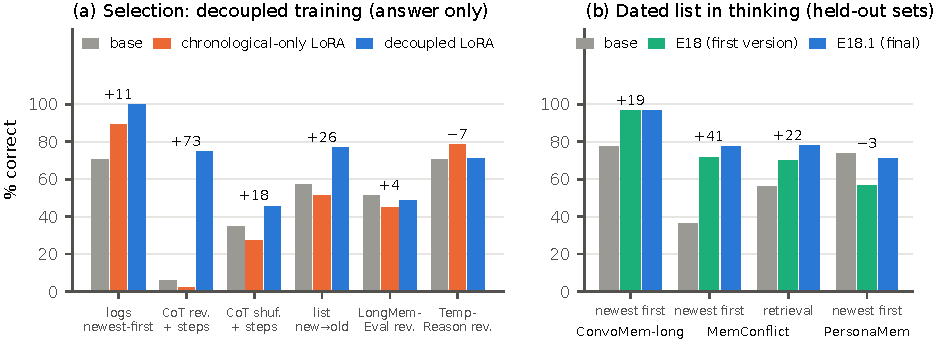
\includegraphics[width=\linewidth]{figures/fig5_fix.pdf}
  \caption{\textbf{Two fixes.} (a) Selection: decoupled versus chronological-only answer-only LoRA (Qwen3-4B, pre-registered); numbers are decoupled minus control. Transfer to unseen formats, failure on LongMemEval sessions and a cost on TempReason. (b) Binding: fact--time training with chronological-only or decoupled block order; both repair held-out ConvoMem-long. Bars marked \emph{pending} are running.}
  \label{fig:fix}
\end{figure}

\subsection{Thinking mode}
Combining thinking mode with the answer-only decoupled LoRA raises newest-first LongMemEval accuracy from 52.6\% to 62.8\% ($+10.3$\ci{0.0}{20.5}; control 42.3\%), short of our pre-registered $+15$. The thinking itself changes little (the newer date is still mentioned first in 69\% of newest-first traces, versus 82\% without the LoRA); most of the gain comes from reading the answer off the thinking (answers agree with the thinking's conclusion in 74\% versus 58\% of items).

% =====================================================================
\section{Discussion and limitations}
\label{sec:discussion}

\paragraph{What the model does.}
Our results suggest a reading strategy that is reasonable for the data models are trained on: when several values compete, take the one written last, because text is almost always written in the order things happen. Explicit time is used when it is local and salient (Qwen3-14B with step numbers in short lists), but in long contexts it is neither bound to the facts nor allowed to override position. The strategy fails exactly when presentation order and time disagree and a conflicting older state is present, which is common in deployed systems.

\paragraph{Practical implications.}
Memory and retrieval pipelines should present retrieved evidence in chronological order whenever timestamps are available; on MemConflict this recovers 19 points at no cost. Clients that show newest-first threads or logs to a model should reverse them. Statements about the order, instructions to reason, and thinking mode are not substitutes.

\paragraph{Limitations.}
\begin{itemize}
  \item \textbf{Scale.} Our largest models have 14B parameters. Qwen3-14B resists explicit step numbers in short contexts but not newest-first LongMemEval sessions ($-24.4$ points). Experiments with 32B--70B models and API models are planned.
  \item \textbf{Seeds and exploratory status.} The selection fix is pre-registered but reported for one seed; the confirmation seeds are paused. The mechanism experiments and the binding fix are exploratory, with thresholds written before running.
  \item \textbf{Judges and parsing.} Free-text answers are graded by Qwen3-14B (91\% agreement with string matching where both apply). For PersonaMem we corrected a parser after seeing that it failed on answers ending in ``The best answer is (d).''; the rule uses only the format, and no prediction of the base models changed.
  \item \textbf{Constructed orders.} Newest-first presentation is constructed by us, although it mirrors common interfaces; retrieval order is not, and it already costs 19 points.
  \item \textbf{Long contexts remain unsolved.} At 25k tokens, writing a dated list first truncates and omits evidence, and neither fix brings LongMemEval to its chronological accuracy.
\end{itemize}

% =====================================================================
\section{Conclusion}
Language models treat ``written later'' as ``happened later''. The default is cheap and usually right, which is why it survives explicit dates, step numbers, ordering statements, retractions and thinking. It fails whenever presentation order and time disagree and a conflicting older state is present---in newest-first threads, in retrieval-ranked memories, and in the model's own reasoning about them. The failure has two parts, selecting the newer value and binding facts to their dates, and each can be trained into the model without seeing the formats where it is tested.

\bibliographystyle{plainnat}
\bibliography{refs}

% =====================================================================
\appendix

\section{Pre-registered thresholds and outcomes}
\label{app:scorecard}

Thresholds were written in \texttt{EXPLORE\_PLAN.md} or \texttt{PREREG\_TRAINING.md} before each run. All experiments are Qwen3-4B, seed 0, unless noted. ``Met'' and ``not met'' refer to the written threshold.

\begin{center}\small
\begin{tabular}{@{}p{0.27\linewidth}p{0.36\linewidth}p{0.3\linewidth}@{}}
\toprule
Experiment & Threshold (written before running) & Outcome \\
\midrule
Selection LoRA, primary endpoint & LongMemEval newest first: decoupled $\geq$ control $+10$, CI $>0$ & \textbf{Not met} ($+3.8$) \\
Selection LoRA, transfer & two further test families, CI $>0$ & Met (logs, CoT, MAB) \\
Selection LoRA, side effects & chronological conditions drop $\leq$2 & Met; TempReason $-7.0$ vs.\ control \\
E1 prefilled timelines & newest-first input raises stale rate $\geq$15 for both models & Met ($+28.6$ each) \\
E1c thinking (first reading) & thinking conclusions $\geq$15 more stale & Not met; \textbf{corrected} by swap experiment (grader read only the last 800 characters) \\
E1c swap & answer follows thinking & Met \\
E1d sorted timeline instruction & stale rate $\geq$15 below the plain timeline prompt and gap to chronological $\leq$5 & Not met (gap $+21.8$) \\
E2 list reading, Qwen3-4B & decoupled $\geq$ control $+10$ & Met ($+25.7$; own timeline $+19.2$) \\
E2 list reading, Phi-4-mini & same & Met ($+27.1$) \\
E3 zeroing recency heads & drop $\geq$2$\times$ random and $\geq$10 & Not met; confounded (reading also breaks) \\
E4 primacy at length & first-value rate $+20$ up to 19k tokens & Not met (0\%) \\
E5 CoT-only LoRA & $\geq$10 on two application tests & Met; LongMemEval reversed ($-20.5$) \\
E7 probes, short contexts & $\geq$80\% on stale-answered items & Met (100\%, $n=13$) \\
E7 probes, long sessions & $\geq$80\% or $\leq$60\% & Inconclusive (69\%) \\
E10 attention routing (oracle) & $+15$ on a long-dialogue set & Met (LongMemEval $+20$) \\
E11 answer from notes only & $\geq$ thinking $+15$ & Not met \\
E12 reasoning LoRA & ConvoMem newest first $\geq$ control $+10$ and base $+10$ & Not met ($+2.4$ / $+9.7$) \\
E13 binding, mechanism & both dates named $\geq$50\% & Met (82.1\%) \\
E13 binding, primary & decoupled $\geq$ control $+10$ and base $+10$ & Half met: base $+17.7$, control $-0.8$ \\
E13 binding on MemConflict & a binding arm $\geq$ base $+10$, chron.\ drop $\leq$5 & \pending{} \\
E14 thinking + LoRA & $\geq$ base thinking $+15$ & Not met ($+10.3$) \\
New long-dialogue sets & newest first $\leq$ chron.\ $-10$, CI $<0$ & ConvoMem-long met; PersonaMem not \\
External sets & same & MemConflict met; LoCoMo not (predicted); MAB-CR untestable \\
\bottomrule
\end{tabular}
\end{center}

\section{PersonaMem diagnostics}
\label{app:pmdiag}

Table~\ref{tab:pm} reports accuracy without the history (\emph{bare}: final user message and options; \emph{no history}: persona, message and options) and with the full history in both orders. By the threshold written in advance, a question type ``does not depend on the history'' if chronological accuracy exceeds no-history accuracy by less than 10 points or the interval includes zero. ``How did the preference evolve'' questions do not depend on the history for either model. For ``why did it change'' questions, Qwen3-4B's no-history condition is 12.1\ci{4.0}{20.2} points below the full history, which formally counts as dependence; the bare condition (80.8\%), however, is within 3 points of the full history, and the persona text lowers accuracy. We note that this reading was made after seeing the results.

\begin{table}[h]
\centering\small
\caption{PersonaMem 32k accuracy (\%) by question type. Bare / no history / chronological / newest first.}
\label{tab:pm}
\begin{tabular}{@{}lrcc@{}}
\toprule
Question type & $n$ & Qwen3-4B & Phi-4-mini \\
\midrule
Track preference evolution & 139 & 56.8 / 58.3 / 62.6 / 67.6 & 51.8 / 51.8 / 51.8 / 51.1 \\
Reasons behind updates & 99 & 80.8 / 71.7 / 83.8 / 82.8 & 68.7 / 70.7 / 73.7 / 73.7 \\
Recall user-shared facts & 129 & 40.3 / 48.1 / 59.7 / 56.6 & 31.0 / 41.1 / 46.5 / 48.1 \\
Recall facts mentioned & 17 & 11.8 / 17.6 / 58.8 / 52.9 & 41.2 / 41.2 / 70.6 / 70.6 \\
Generalize to new scenarios & 57 & 21.1 / 38.6 / 63.2 / 57.9 & 17.5 / 28.1 / 43.9 / 38.6 \\
Preference-aligned recommendations & 55 & 40.0 / 23.6 / 58.2 / 61.8 & 34.5 / 34.5 / 47.3 / 47.3 \\
Suggest new ideas & 93 & 12.9 / 10.8 / 10.8 / 9.7 & 15.1 / 12.9 / 22.6 / 17.2 \\
\bottomrule
\end{tabular}
\end{table}

\section{Test-set construction}
\label{app:sets}

\paragraph{ConvoMem-long.} ConvoMem changing-evidence items with two evidence conversations, personas 50--99, four items per persona (124 items). Both full conversations are shown, headed ``Conversation (date: \ldots)'' with dates drawn so that the earlier conversation in the source gets the earlier date; a ``Current date'' line follows, and the model answers in one sentence.

\paragraph{MemConflict.} From the released benchmark file (30 simulated users), dynamic-conflict questions of medium difficulty whose reference answer names both the old and the new value of exactly one changed attribute. We keep a question only if the old value does not occur in the update session and does occur in an earlier session (structural filter, no model outputs used), take the latest such session, the update session and the sessions immediately before the update up to about 20k source tokens, and sample at most 8 questions per user. A few malformed messages in the source (28 of 142k) are rendered by their available text.

\paragraph{PersonaMem.} PersonaMem-v1, 32k contexts. The context up to the question is split into sessions at the persona system message; sessions receive increasing dates in source order and are shown oldest or newest first; four-way multiple choice.

\paragraph{LoCoMo.} All 321 temporal questions (category 2) over the full conversations, each session headed by its original date and time.

\paragraph{Retrieval order.} BM25 ($k_1 = 1.5$, $b = 0.75$) between the question and each session (or fact), computed within each item; ties keep source order.

\section{Training data details}
\label{app:train}
\note{To be expanded: generators \texttt{gen\_train\_data.py} (selection) and \texttt{gen\_bind\_data.py} (binding); data hashes; development-set curves; the full pre-registration with its change log.}

\end{document}
